\section{Introduction}
\label{sec:intro}

% Talks about how AUV missions are traditionally planned. Why they might have
% been adequate in the past and are no longer so. How can deliberation
% (i.e. planning help) and how can it contribute to new ways of observing the
% ocean.

Autonomous platforms in the marine environment have had a substantial
and immediate impact for both civil and military
applications. Autonomous Underwater Vehicles (AUVs) have not only
altered the ability of oceanographers to reach beyond the surface and
make high resolution observations, but have impacted the engineering
methodologies behind sampling, control and robotics itself
\cite{Brierley08032002,ryan05,Thomas06,Yoerger01012007,Incze2009,Rigby10}. Yet
challenges remain, principally in making such robotic devices more
attune to the environment, to sample large swaths at the Meso-scale
($> 50$ km\textsuperscript{2}) and doing so systematically and
adaptively. Further, over the last two decades substantial
improvements in hardware including propulsion and battery technologies
have outpaced software especially in algorithmic methods in sampling
and control and in systematic software engineering development.

Large scale high resolution observations have become increasingly
tractable using autonomous platforms both on and below the surface.
This, in turn, has lead to periodic calls for sustained exploration
and sampling \cite{rudnick03}, illustrating the high scientific value
placed on such data.  The complexity of oceanic processes and the
chronic under-sampling of the coastal oceans, especially of dynamic
features studied over a variety of spatial and temporal scales, has
made it challenging for robotic platforms to autonomously track and
sample. A prominent example of such a process is coastal algal blooms
which are patchy and could cover large coastal zones. Persistent
observation of such dynamic events dictates that our robotic assets
track and sample such patches which can evolve rapidly due to inherent
bio-geochemical activity, as well as advection and diffusion of the
water mass it resides in.

At the Monterey Bay Aquarium Research Institute (MBARI), a unique
inter-disciplinary collaboration between biologists, ecologists,
geneticists and roboticists on the \can (Controlled Agile Novel
Observation Network) program \cite{canon} has driven autonomous system
exploration and control. Fundamental questions related to sampling
strategies have driven the use cases for advanced concepts in
autonomy, specifically to Artificial Intelligence (AI) Planning and
Execution. Current work is also looking at how other fields in Machine
Intelligence especially Machine Learning can be leveraged to impact
the science of engineering systems in marine robotics and as a
consequence oceanography itself.

In this chapter, we propose an alternative view to decision-making
using in-situ automated Planning \cite{ghallab04}. More importantly,
we demonstrate that earlier control paradigms (primarily driven by
\emph{reactive} approaches to control) can be augmented to provide
targeted observation and sampling as well as a more nuanced and
balanced consideration of mission objectives, environmental conditions
and available resources. Planning (or deliberation or projection in
action space \kcomment{and used interchangeably in this chapter}) is
important to balance current needs of a robot with future desires or
goals taking into account time and available resources in-situ on the
robot. Planning without time or action planning in and of itself is
not adequate; dealing with time ensures that the balance between now
and the future is handled systematically. Yet, plans have to be tied
to robotic action and in the real-world which is not static. Further,
plans project future state which is not only likely to change, but is
based on substantial uncertainty\footnote{It is important to remember
  that these principles are broad much as Dwight Eisenhower is reputed
  to have said ``\emph{In preparing for battle I have always found
    that plans are useless, but planning is indispensable}'' and
  ``\emph{Failing to plan is planning to fail}''}. Use of
environmental cues is often hampered by poor \kcomment{predictive}
skill \cite{anderson2009} of ocean models and little to no
availability of a priori synoptic views of the survey
area. \kcomment{Planning therefore provides a ``buffer'' against the
  stochastic environment.}


AUV control architectures have primarily been driven by reactive
Subsumption-based approaches \cite{brooks86}. They have been adequate
to doing routine straight-line survey trajectories which have played a
valuable role in the acceptance of AUVs as a new tool for ocean
science and DoD applications. However, scaling of problem domains in
addition to dealing with event-response and discovery in the
water-column challenges \emph{how} controllers are written in the
first place, maintained and upgraded over the life-cycle of the
platform. Dealing with off-nominal endogenous or exogenous conditions
including sensor failures stretches how AUVs are currently being
utilized; one consequence for instance, is any off-nominal condition
results in a \emph{fail-safe} surface mode to radio for help. Software
design using these reactive approaches, not only makes it hard for
sustaining engineering development, these approaches are not
adequately adaptive for emerging ocean science problems.  Despite
vigorous defense by Brooks early on
\cite{Brooks91intelligencewithoutrea,Brooks91intelligencewithoutrep},
autonomous systems require a model if not of the world then of the
\emph{physics} of the vehicle when it interacts with the world.


Criticism of AI planning, on the other hand, also well articulated by
Brooks, was targeting the performance of in-situ
deliberation. Terrestrial robotic platforms were well-known to
frequently stop and ``plan''; assuming in the meantime that the world
will remain static. In the marine robotics world, such a situation
would simply not be permissible given the need to make continuous
observations without stopping an under-articulated robotic platform
such as an AUV. However, algorithmic and implementational advances by
the AI community over the years have produced a range of planners with
demonstrated embedded capabilities
\cite{simmons94,Haigh98,alami:1998p820,chien00,mus98,teichteil07}. Our
work has been influenced by and in turn influenced a wide range of
activities in the field of AI Planning and Plan Execution with
demonstrated real-world and highly visible capabilities in the Space
domain \cite{mus98,rajan00,aichang04,bresina05} for NASA. Lessons
learned have been applied to the world of marine robotics which we
bring together in this chapter. Important lessons that were derived
from this rich legacy included the following:

\begin{itemize}

\item Projecting plans (or using \emph{deliberation}) can and should
  balance near-term objectives with end-term or even evolving goals.

\item Dealing with time and resources is essential in real-world
  planning.

\item A rich representation that can deal with co-temporal events for
  modeling complex systems is a must.

\item Fast solvers for incremental causal reasoning can be built as a
  basis for dealing with dynamic controllable events where replanning
  is tightly integrated.

\item Planning should be tightly inter-leaved with execution to enable
  responsiveness to events which impact plan failure. This is also an
  important factor leading to platform adaptivity.

\item A model-based approach should separate control formulation of
  the platform which describes operational characteristics, from the
  domain. The controller can then be rigorously tested and certified
  even as the domain model evolves to fit diverse applications.

\end{itemize}

We have developed, tested and deployed the Teleo-Reactive EXecutive
(\rxe) an on-board adaptive control system that integrates AI based
planning and state estimation in a hybrid
executive\cite{mcgann08a,mcgann08b,py10}.  State estimation allows the
system to keep track of world evolution as time advances based on a
formal model distributed through the architecture.  Onboard planning
and execution enables adaptation of navigation and instrument control
based on the state identified during state estimation.  It further
enables goal-directed commanding within the context of projected
mission state and allows for replanning for off-nominal situations and
opportunistic science events. The framework in addition to being used
on an AUV, is general enough \kcomment{to} be used for controlling a
personal robot \cite{pr2,Meeussen:2010dn,mcgann2009} and is deployed
on a European planetary rover testbed \cite{goac11}. While it is
possible to integrate probabilistic estimation on top of this
framework \cite{mcgann08d}, such representation is not explicitly
handled by the framework and is out of scope of this chapter.
Deliberation and reaction are integrated systematically over different
temporal and functional scopes within a single agent and a single
model that covers the needs of high-level mission management,
low-level navigation, instrument control, and detection of
unstructured and poorly understood phenomena. \rx is deployed on
MBARI's \emph{Dorado} AUV shown in Fig. \ref{fig:auv-fig}, which to
the best of our knowledge is the only operational marine platform
anywhere being used for routine scientific surveys with onboard plan
synthesis.

\begin{figure}[t]
  \centering \vskip-5pt
  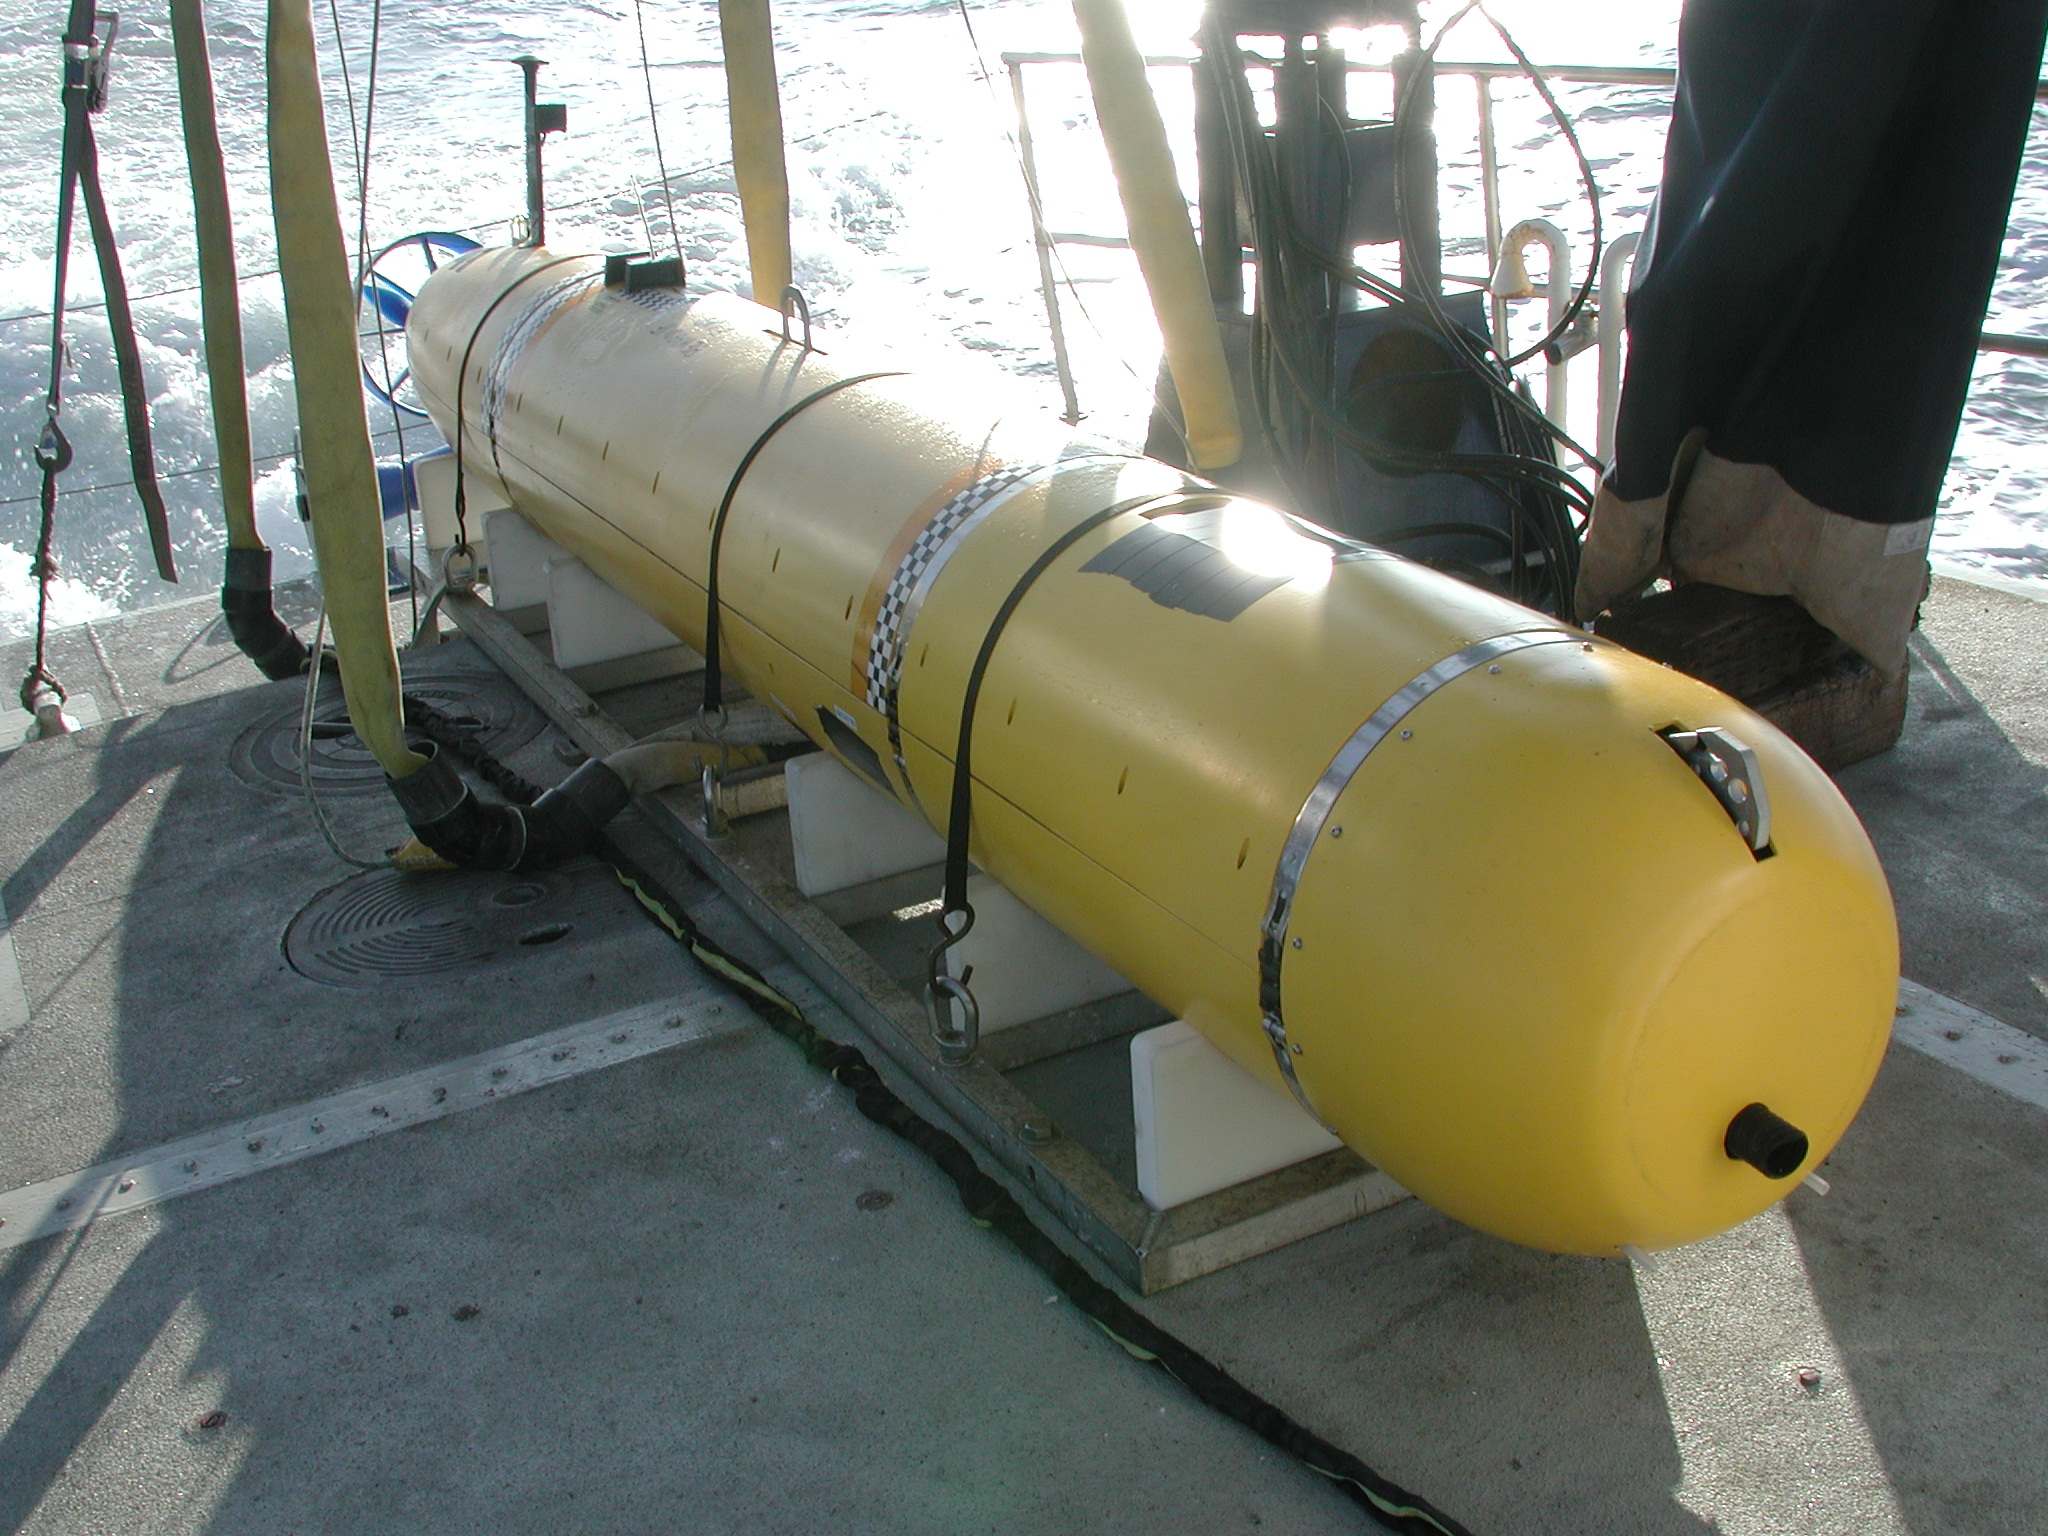
\includegraphics[scale=0.1]{figs/MBARI-AUV.jpg}
  \caption{\small The MBARI \emph{Dorado} AUV on its support vessel
    the R/V \emph{Zephyr}.}
  \label{fig:auv-fig}
  \vskip-0.3cm
\end{figure}

This chapter is organized as follows. We start with some foundational
concepts in our Planning framework in Section~\ref{sec:concepts} which
includes a brief overview of AI Planning in
Section~\ref{sec:planningfound}. In Section~\ref{sec:basics} we go
deeper into the \eu framework itself, the basis of all deliberation
within \rxe. A key portion is Section~\ref{sec:europa:pr} which
details the internal plan representation within a situated agent like
\rxe. Modeling (Section~\ref{sec:europa:modeling}), Inference
(Section~\ref{sec:europa:inference}) and Search
(Section~\ref{sec:europa:search}) articulates important details
associated with \eu critical to \rxe.  With these foundational
elements of deliberation out of the way, we transition to \rx itself
in Section~\ref{sec:arch}, bring out architectural details in
Section~\ref{sec:arch:trex}, deal with the execution cycle in
Section~\ref{sec:arch:exec}, highlight how \rx deliberates in
Section~\ref{sec:arch:europa}, finally delving deeper into the key
concept of synchronization in Section~\ref{sec:arch:synch}. Further
details on deliberation within \rx (Section~\ref{sec:arch:plan}) and
how planning and execution are interleaved are shown in
Section~\ref{sec:arch:intertwine}. We offer results from our
experiments at sea in Section~\ref{sec:results}, offer some insights
into the near-term future goals of our research in
Section~\ref{sec:future} and conclude with
Section~\ref{sec:conclusion}.

%%% Local Variables: 
%%% mode: latex
%%% TeX-master: "setobook"
%%% End: 
